
\chapter{Background Theory}

\label{ch:background}

\section{Introduction}
Galaxy morphology has traditionally been classified based on the Hubble sequence, originating from the identification galaxy features from photographic plates. However, this classification is based on visual distinctions and fails to accurately represent early-type galaxies (E's and S0's) and it was argued by \cite{Cappellari2011} and \cite{Emsellem2011} that a more telling classification would be based on the spin parameter due to the intrinsic qualitative change in velocity structure exhibited by galaxies, with a threshold of separating slow ($\lambda<0.1$) and fast ($\geq0.1$) rotators, as can be seen below. This threshold was later updated to include the ellipticity $\epsilon$ by defining slow rotators and fast rotators have $\lambda_{Re}$ lower and larger than $k_{FS} \times \sqrt{\epsilon}$, respectively, where $k_{FS} = 0.31$ for measurements made within an effective radius $R_{e}$ \cite{Emsellem2011}. This new criterion is nearly independent of viewing angle.
$\lambda_{R}$ is defined as\cite{sauron9}:
\begin{equation}
\lambda_{R} = \frac{\sum_{i=1}^{N_{p}} F_{i}R_{i}|V_{i}|}{\sum_{i=1}^{N_{p}}F_{i}R_{i}\sqrt{V_{i}^2+\sigma_{i}^2}}
\end{equation}
where $F_i$, $R_i$, $V_i$ and $σ_i$ are the flux, circular radius, velocity and velocity dispersion of the ith spatial bin, the sum running on the $N_p$ bins. $\lambda_{Re}$ indicates spin parameter calculated within 1 effective radius $R_{e}$.
This is superior over a velocity dispersion classification, $V/\sigma$, which fails when confronted by galaxies with kinematically decouple cores (KDC), "whose angular momentum vector is misaligned with respect to that of the bulk of the galaxy" \cite{mo_bosch_white_2010}. Furthermore, $\lambda_{R}$ 'can quantify galaxy morphology via the kinematic properties of galaxies\cite{Cortese2016}', beyond early types. 
\begin{figure}[h]
	\centering
	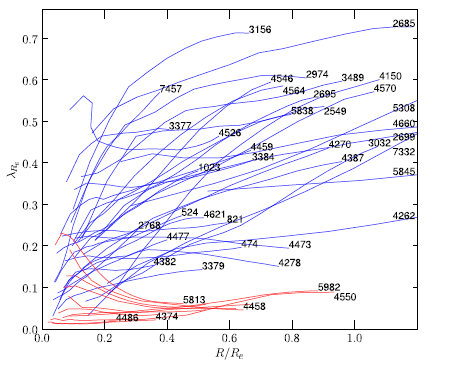
\includegraphics{fastslowemsellem2008.png}
	\caption{Radial $\lambda_{R}$ profiles for the 48 E and S0 galaxies of the SAURON
		sample. Profiles of slow and fast rotators are coloured in red and blue, respectively.
		NGC numbers are indicated for all fast rotators and most slow.
		rotators \cite{Emsellem2011}}
	\label{fig:morphsplit}
\end{figure}

\begin{figure}[h]
	\centering
	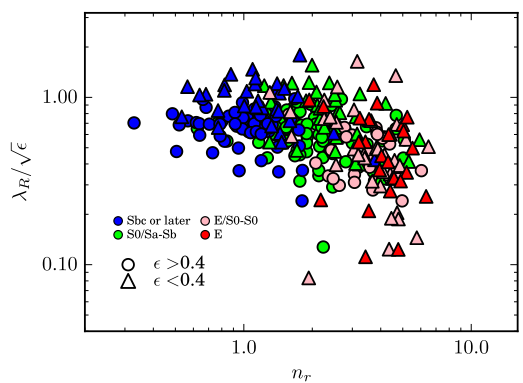
\includegraphics{morphology_sersic_cortese2016.png}
	\caption{Galaxies from ATLAS$_{3D}$ colour coded by optical morphology. There appears a weak correlation for early types that grows more pronounced for late types (Sbc or later), using se\'rsic index as a weak proxy for morphology.	
		\cite{Cortese2016}}
	\label{fig:morphologysersic}
\end{figure}
As can be seen in figure \ref{fig:morphologysersic}, there appears a weak correlation for galaxies in the ATLAS$_{3D}$ survey for early-type galaxies, suggesting that based on se\'rsic index alone there is some prospect for applying statistical methods to infer morphology.
The spin parameter is costly to determine due to its reliance on integral field spectroscopy and has therefore only been found for a small number of galaxies: 260 from the ATLAS3D survey and 446 from SAMI. This compares with over 500 million galaxies with photometric data from the Sloan Digital Sky Survey (SDSS) alone \cite{SDSS}. Although other classifications do not rely on this parameter, it is still of value in relation to other properties. It is therefore of great value to find an alternative means of identifying the rotation.\
Although the motivation for this study is to extend identifying the spin parameter to all morphological classes, this paper will focus on the early-type galaxies taken from \cite{Emsellem2011}, defined as Hubble type E/S0's, T-type $T < −3.5$ (Es) and $T \geq −3.5$ (S0s).
\section{Variations of the Spin Parameter}
The ATLAS3D paper measured $\lambda$ to 1 effective radius, $R_{e}$ and to half the effective radius, $R_{e}/2$, where 
\begin{equation}
I(R_{e}=I_{0}/e)
\end{equation}
The spin parameter was later updated by \cite{Cappellari2011} to take account of possible line-of-sight dependencies on the orientation by including the ellipticity, and thus was defined as:
\begin{equation}
\lambda_{Re} = \frac{\lambda}{\sqrt{\epsilon}}
\end{equation}
and hence the threshold for separating fast and slow rotators was defined as:
\begin{equation}
\lambda_{Re}=(0.31\pm0.01)\times \sqrt{\epsilon}
\end{equation}
\section{S\'ersic Index of the Single Fit and Bulge Component, n and n$_{b}$}
The S\'ersic profile models the light intensity over the surface of the galaxy in terms of an exponential function as a function of the distance from the centre, R, and the S\'ersic index n:
\begin{equation}
I(R) = I_{e} exp\{-b_{n} [(R/R_{e})^{1/n}-1]\}
\end{equation}
As such, this parameter is one way of quantifying the morphological differences between structurally distinct galaxies. The light will vary dependent on the different populations of stars and their distribution throughout the galaxy.
\begin{figure}[h!]
	\centering
	\begin{subfigure}{.5\textwidth}
		\centering
		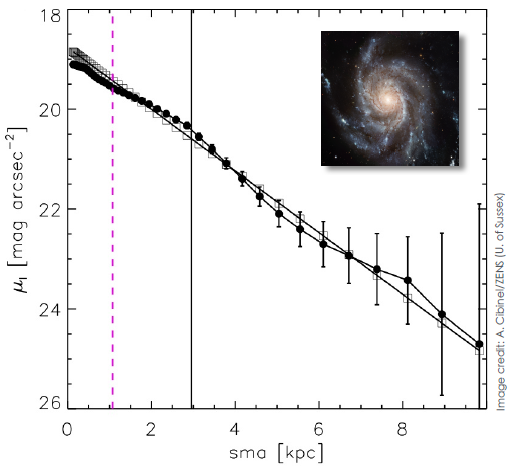
\includegraphics[width=.6\linewidth]{sersic_disks_from_lectures.png}
		\caption{Late-type Spiral Galaxy}
		\label{fig:sub1}
	\end{subfigure}%
	\begin{subfigure}{.5\textwidth}
		\centering
		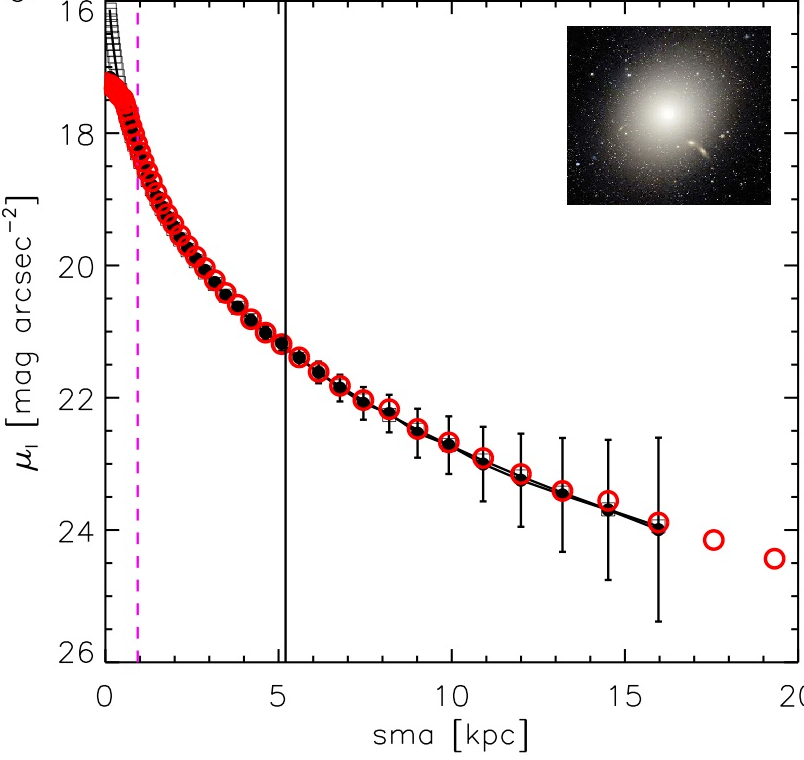
\includegraphics[width=.6\linewidth]{sersic_elliptical_from_lectures.png}
		\caption{Early-Type Elliptical Galaxy}
		\label{fig:sub2}
	\end{subfigure}
	\caption{Se\'rsic Index as a Descriptor of Morphology}
	\label{fig:test}
\end{figure}

\section{Disk-to-Total Light Ratio, D/T}
This measures the proportion of light from the galaxy that emanates from the disk compared to the total light measured from the galaxy.
\begin{figure}[h!]
	\centering
	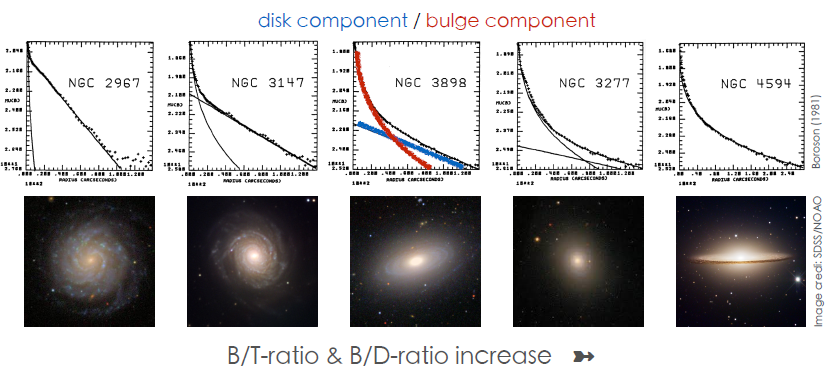
\includegraphics[width=\textwidth]{DT_example_from_lectures.png}
	\caption{The D/T ratio measures how much of a galaxies light is distributed throughout the disk compared to the total light. Late-types have more pronounced spiral arms and so have a larger D/T value. \cite{Lectures}
	}
	\label{fig:dtexample}
\end{figure}

\section{ATLAS$^{3D}$}
According to \cite{Cappellari2011}, this survey focused on a 'volume-limited ($\num{1.16e05} Mpc^{3}$) sample of 260 early-type (elliptical E and lenticular S0) galaxies (ETGs)...The sample consists of nearby (D < 42 Mpc, $|\delta \num{-29}^{\circ}| < 35^{\circ}$, $|b| > 15^{\circ})$ morphologically selected ETG's extracted from a parent sample of 871 galaxies (8 per cent E, 22 per cent S0 and
70 per cent spirals) brighter than $M_{K} <\num{-21.5} $mag (stellar mass $M_{\star} \gtrsim \num{6e09} M_{\odot}$).' ETG's were defined as having de Vaucouleurs T type T > -3.5 and T $\leq -3.5$ for S0 and E galaxies respectively, which correlates with the Hubble classes lenticular and elliptical.


